% =====================================================================
% Capítulo 2: Marco Teórico y Estado del Arte
%   Este archivo:          Secs. 2.1-2.6 (co-agrupamiento de Bregman y ST-CC)
%   Cap_Estadistica.tex:   Secs. 2.7-2.8 (pruebas de hipótesis y SigTree)
%   Cap_EA.tex:            Secs. 2.9-2.10 (estado del arte y cierre)
% =====================================================================

\chapter{Marco Teórico y Estado del Arte}\label{chap:marco}

Este capítulo reúne los fundamentos sobre los que se construye la propuesta y la
revisión de los trabajos relacionados. Tiene dos partes. La primera, el marco
teórico, reúne dos líneas que la propuesta combina, a saber, el co-agrupamiento
de matrices espacio-temporales y las pruebas de hipótesis sobre tablas de
conteo. La segunda revisa los trabajos publicados desde 2020 y señala la brecha que aborda
esta tesis.

El marco teórico avanza de lo general a lo específico. Primero se describe cómo
los datos espacio-temporales se organizan en una matriz de co-ocurrencia y qué
tipos de estructura de bloques pueden imponerse sobre ella
(Secciones~\ref{sec:matriz} y~\ref{sec:estructuras}). Luego se introducen las
divergencias de Bregman, que permiten tratar con una sola formulación funciones de
pérdida tan distintas como la distancia euclídea y la divergencia de
Kullback--Leibler (Sección~\ref{sec:bregman}). Sobre ellas se construye el marco
general de co-agrupamiento de \cite{Banerjee2007}, con sus seis bases de
aproximación (Sección~\ref{sec:bbac}). El capítulo se detiene en el caso de la
I-divergencia, donde el co-agrupamiento admite una lectura exacta como ajuste de
modelos de Poisson y la divergencia se descompone en términos interpretables
(Sección~\ref{sec:idiv-poisson}). Esa descomposición es la base del criterio de
refinamiento que propone esta tesis. A continuación se describe el marco ST-CC de
\cite{Liu2021} (Sección~\ref{sec:stcc}). La parte estadística presenta las pruebas
de independencia y su calibración, el control de comparaciones múltiples, la
inferencia después de la selección y el tamaño de efecto
(Sección~\ref{sec:pruebas}), y cierra con SigTree \cite{Hu2025}, el algoritmo de
agrupamiento guiado por pruebas de hipótesis del que la propuesta toma su
criterio de parada (Sección~\ref{sec:sigtree}). Finalmente, la
Sección~\ref{sec:estado-arte} presenta el estado del arte.

% ---------------------------------------------------------------------
\section{Datos espacio-temporales y matriz de co-ocurrencia}\label{sec:matriz}

Los datos de movilidad urbana se registran como eventos individuales. Cada viaje
en taxi, por ejemplo, queda descrito por el lugar y el instante en que el pasajero
sube y baja del vehículo. Para analizarlos de forma agregada, el espacio se divide
en $m$ regiones fijas, y el día se divide en $n$ intervalos de igual duración. En la
clasificación de \cite{Wu2020}, el resultado es una serie temporal
georreferenciada, es decir, un conjunto de valores observados en ubicaciones fijas y a
intervalos regulares, que puede organizarse como una matriz bidimensional.

\subsection{La matriz de co-ocurrencia}

Sea un periodo de observación de $D$ días. La matriz de co-ocurrencia
$O \in \mathbb{N}^{m \times n}$ tiene como entrada $O_{ij}$ el número de eventos,
por ejemplo llegadas de taxi, registrados en la región $i$ durante el intervalo
$j$, sumados sobre los $D$ días. Cada fila de $O$ es el perfil temporal de
una región, es decir, cómo se reparte su actividad a lo largo del día, y cada
columna es el perfil espacial de un intervalo, es decir, cómo se reparte la
actividad de ese horario entre las regiones. Se denotan
$O_{i\cdot} = \sum_j O_{ij}$, $O_{\cdot j} = \sum_i O_{ij}$ y $N = \sum_{i,j} O_{ij}$
los totales de fila, de columna y general. Se denota además $X_{dij}$ el número
de eventos de la región $i$ en el intervalo $j$ durante el día $d$, de modo que
$O_{ij} = \sum_{d=1}^{D} X_{dij}$. Las $D$ matrices diarias $X_d$ son réplicas
de un mismo periodo, y permiten medir cuánto varían los conteos de un día a
otro sin suponer un modelo para esa variación.

\cite{Liu2021} interpretan esta matriz como la distribución de co-ocurrencia de dos
variables aleatorias, la región $R$ y el intervalo $T$. Al dividir entre el total
se obtiene la distribución conjunta empírica
\begin{equation}\label{eq:conjunta}
  p(r_i, t_j) = \frac{O_{ij}}{N}, \qquad
  p(r_i) = \frac{O_{i\cdot}}{N}, \qquad
  p(t_j) = \frac{O_{\cdot j}}{N},
\end{equation}
que describe la probabilidad de que un evento elegido al azar ocurra en la región
$r_i$ y en el intervalo $t_j$. La dependencia entre dónde y cuándo ocurren los
eventos se mide con la información mutua \cite{Cover2006},
\begin{equation}\label{eq:im}
  I(R;T) = \sum_{i,j} p(r_i,t_j) \log \frac{p(r_i,t_j)}{p(r_i)\,p(t_j)} ,
\end{equation}
que es no negativa y se anula si y solo si
$O_{ij} = O_{i\cdot}\,O_{\cdot j}/N$ para todas las celdas. En ese caso todas las
regiones tienen el mismo perfil temporal, salvo un factor de escala, y conocer la
región no aporta información sobre el horario. Cuanto mayor es $I(R;T)$, más
depende el ritmo diario de cuál sea la región. Esta interacción entre
espacio y tiempo es precisamente lo que buscan revelar los métodos de
co-agrupamiento.

\subsection{Modelo de conteos}\label{sec:modelo-conteos}

ST-CC no adopta ningún modelo probabilístico, sino que optimiza una función de
pérdida y elige el número de grupos con criterios heurísticos (Sección~\ref{sec:stcc}).
Para someter sus bloques a pruebas de hipótesis, como propone esta tesis, se
necesita un modelo de cómo varían los conteos. El modelo de referencia para
conteos de eventos es el de Poisson, en el que se supone que
$O_{ij} \sim \mathrm{Poisson}(\mu_{ij})$, con conteos independientes entre celdas.
En este modelo la media y la varianza de cada conteo coinciden,
$\mathrm{E}[O_{ij}] = \mathrm{Var}(O_{ij}) = \mu_{ij}$, de modo que el ruido
relativo de una celda, $1/\sqrt{\mu_{ij}}$, disminuye a medida que crece su
actividad. La justificación es que cada conteo agrega un número muy grande de
decisiones de viaje individuales, cada una con una probabilidad pequeña,
constante e independiente de las demás, de caer en una celda concreta, que es la
situación en que la distribución de Poisson aproxima a la binomial. Si además se
condiciona sobre el total $N$, el vector de conteos sigue una distribución
multinomial con probabilidades $\pi_{ij} = \mu_{ij}/\sum_{k,l} \mu_{kl}$. Para
los modelos log-lineales que incluyen un término para el total, como todos los
que se usan en esta tesis, ambos esquemas de muestreo conducen a las mismas
estimaciones de máxima verosimilitud para las probabilidades $\pi_{ij}$
\cite{Agresti2013}. Por eso la distribución empírica~\eqref{eq:conjunta} puede
leerse como la estimación de $\pi$ bajo cualquiera de los dos modelos.

Este modelo tiene dos limitaciones que se retoman más adelante. La primera es que
los supuestos de la justificación no se cumplen del todo. La probabilidad de
viajar no es constante, ya que la actividad de una celda varía de un día a otro por el
día de la semana, el clima o los eventos puntuales, lo que produce más
variabilidad de la que predice el modelo de Poisson
(Sección~\ref{sec:est-efecto}). Además, esos factores actúan sobre muchas celdas
a la vez; un día de lluvia, por ejemplo, aumenta la actividad en casi todas las
regiones, de modo que los conteos de celdas distintas tampoco son del todo
independientes. La Sección~\ref{sec:prop-sobredispersion} constata ambos efectos
en los datos de esta tesis. La segunda es que la equivalencia entre el
co-agrupamiento con I-divergencia y la verosimilitud de Poisson exige que las
celdas contengan conteos y no promedios, lo que se analiza en la
Sección~\ref{sec:escala}.

% ---------------------------------------------------------------------
\section{Co-agrupamiento y estructuras de bloques}\label{sec:estructuras}

El agrupamiento tradicional, llamado también agrupamiento unidireccional, forma
grupos en una sola dimensión de la matriz, a partir de la similitud de los datos a
lo largo de la otra \cite{Wu2020}. Aplicado a la matriz $O$, agrupa regiones según
sus perfiles temporales completos, o intervalos según sus perfiles espaciales
completos. El co-agrupamiento forma grupos en las dos dimensiones a la vez,
de modo que cada grupo de filas se describe por su comportamiento en cada grupo de
columnas \cite{Wu2020}. La idea se remonta al agrupamiento directo de
\cite{Hartigan1972}, considerado el origen del \emph{biclustering} \cite{Castanho2024}.
Dependiendo de las restricciones que se imponen sobre la forma de los grupos, se
obtienen estructuras de bloques muy distintas. La
Figura~\ref{fig:estructuras} y la Tabla~\ref{tab:estructuras} resumen las que son
relevantes para esta tesis.

\begin{figure}[t]
\centering
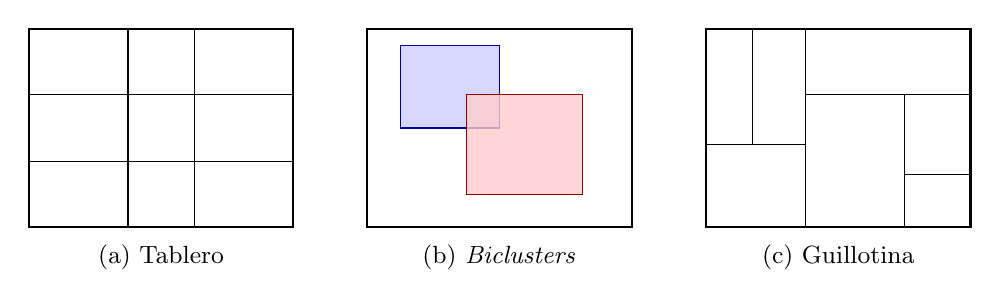
\begin{tikzpicture}[x=0.42cm,y=0.42cm]
  % (a) tablero
  \begin{scope}
    \draw[thick] (0,0) rectangle (8,6);
    \foreach \x in {3,5} \draw (\x,0) -- (\x,6);
    \foreach \y in {2,4} \draw (0,\y) -- (8,\y);
    \node at (4,-0.9) {\small (a) Tablero};
  \end{scope}
  % (b) biclusters
  \begin{scope}[xshift=4.3cm]
    \draw[thick] (0,0) rectangle (8,6);
    \fill[blue!20, opacity=0.8] (1,3) rectangle (4,5.5);
    \draw[blue!60!black] (1,3) rectangle (4,5.5);
    \fill[red!20, opacity=0.8] (3,1) rectangle (6.5,4);
    \draw[red!60!black] (3,1) rectangle (6.5,4);
    \node at (4,-0.9) {\small (b) \emph{Biclusters}};
  \end{scope}
  % (c) guillotina
  \begin{scope}[xshift=8.6cm]
    \draw[thick] (0,0) rectangle (8,6);
    \draw (3,0) -- (3,6);
    \draw (0,2.5) -- (3,2.5);
    \draw (3,4) -- (8,4);
    \draw (1.4,2.5) -- (1.4,6);
    \draw (6,0) -- (6,4);
    \draw (6,1.6) -- (8,1.6);
    \node at (4,-0.9) {\small (c) Guillotina};
  \end{scope}
\end{tikzpicture}
\caption{Tres estructuras de bloques sobre una matriz región~$\times$~tiempo.
En (a), la partición en tablero, cada corte atraviesa toda la matriz; en (b), los
\emph{biclusters} son submatrices que pueden solaparse y no cubren toda la matriz; y en
(c), la teselación guillotina consiste en cortes recursivos que solo afectan al
bloque donde se producen. Las
filas y columnas se muestran contiguas para simplificar el dibujo; en general
cada grupo es un subconjunto cualquiera de filas o de columnas.}
\label{fig:estructuras}
\end{figure}

\subsection{Partición en tablero}

La estructura más simple particiona las filas en $K_R$ grupos y las columnas en
$K_T$ grupos, de forma que cada celda pertenece a exactamente un bloque
(Figura~\ref{fig:estructuras}a). En la taxonomía de \emph{biclustering} que recoge
\cite{Castanho2024} corresponde a la estructura de filas y columnas exclusivas;
en la literatura de co-agrupamiento se la llama partición en tablero
(\emph{checkerboard}) \cite{Liu2021}. Es la estructura que producen el
co-agrupamiento de teoría de la información \cite{Dhillon2003}, el co-agrupamiento
de Bregman \cite{Banerjee2007} y, por tanto, ST-CC. Su ventaja es la
interpretabilidad, ya que la matriz se resume en $K_R K_T$ bloques, y cada grupo de filas
y de columnas tiene una lectura directa. Su desventaja es que cada división es
global, es decir, que si un grupo de filas se divide, la división se aplica en todos los
grupos de columnas, aunque la diferencia solo exista en uno de ellos.

Dentro de esta familia, una línea de trabajo se ocupa de elegir el número de
bloques de forma automática. Cross-Associations \cite{Chakrabarti2004} particiona
matrices binarias y elige el número de grupos de filas y de columnas con el
principio de longitud de descripción mínima (MDL), sin parámetros del usuario. Los
modelos de bloques latentes, revisados por \cite{Biernacki2023}, tratan la
pertenencia de filas y columnas a sus grupos como variables latentes de un modelo
probabilístico y eligen el número de grupos con criterios de selección de modelo.
En ambos casos el resultado sigue siendo un tablero, pues se decide cuántos
cortes globales hacer, pero no se permite que un corte afecte solo a una parte de
la matriz.

\subsection{\emph{Biclusters}}

El \emph{biclustering} relaja la exigencia de cubrir toda la matriz y busca submatrices,
llamadas \emph{biclusters}, cuyas filas se comportan de forma coherente en sus columnas,
y admite que un mismo elemento pertenezca a varios \emph{biclusters} o a ninguno
(Figura~\ref{fig:estructuras}b) \cite{Castanho2024}. Esta flexibilidad permite
describir patrones locales, pero tiene un costo, pues cuando los \emph{biclusters} se solapan
de forma arbitraria, es más difícil extraer conocimiento del resultado
\cite{Castanho2024}, y el resultado deja de ser una partición de la matriz, por lo
que no puede compararse directamente con un tablero en términos de error de
reconstrucción.

\subsection{Estructuras jerárquicas y teselaciones guillotina}

Una tercera posibilidad es organizar los bloques en una jerarquía. En la versión
más común se construye un dendrograma para las filas y otro para las columnas;
cortar ambos a cierta altura vuelve a producir un tablero, solo que con una
resolución elegida a posteriori. Una alternativa distinta es la teselación
guillotina en la cual se parte de la matriz completa, o de un tablero inicial, y se aplican
cortes recursivos, cada uno de los cuales divide un único bloque en dos por filas
o por columnas (Figura~\ref{fig:estructuras}c). El resultado sigue siendo una
partición de la matriz en rectángulos, en el sentido de subconjuntos de filas por
subconjuntos de columnas, pero ya no es un tablero, porque dos filas del mismo
grupo pueden quedar con particiones temporales distintas.

El proceso de Mondrian de \cite{Roy2008} es la referencia clásica de este tipo de
estructura. Los autores parten de la misma observación que motiva esta tesis, a
saber, que en los modelos de bloques con partición regular, capturar un detalle
fino en una zona de la matriz obliga a dividir toda la fila o columna. Para evitarlo, definen
una distribución de probabilidad sobre árboles de cortes alineados con los ejes, y
la usan como distribución a priori en un modelo bayesiano no paramétrico de datos
relacionales, con inferencia mediante métodos de Monte Carlo. La propuesta de esta
tesis produce el mismo tipo de estructura, pero por una vía distinta, pues parte
del tablero de ST-CC y decide cada corte con una prueba de hipótesis, en lugar de
muestrear la teselación completa de una distribución a posteriori.

\begin{table}[ht]
  \centering
  {\footnotesize
  \renewcommand{\arraystretch}{1.4}
  \begin{tabular}{@{}l c c c >{\raggedright\arraybackslash}p{0.28\textwidth}@{}}
    \toprule
    \textbf{Estructura} & \textbf{Partición} & \textbf{Solapamiento} &
    \textbf{Cortes locales} & \textbf{Ejemplos} \\
    \midrule
    Tablero & Sí & No & No & ITCC, BBAC, ST-CC, Cross-Associations \\
    \midrule
    \emph{Biclusters} & No & Sí & -- & \emph{Biclustering} \cite{Castanho2024} \\
    \midrule
    Jerárquica por dimensión & Sí & No & No & Dendrogramas de filas y columnas \\
    \midrule
    Guillotina & Sí & No & Sí & Proceso de Mondrian \cite{Roy2008}, esta tesis \\
    \bottomrule
  \end{tabular}
  }
  \caption{Comparación de estructuras de bloques. La columna Partición indica si
  cada celda pertenece a exactamente un bloque, y la columna Cortes locales, si
  una división puede afectar solo a una parte de la matriz.}
  \label{tab:estructuras}
\end{table}

% ---------------------------------------------------------------------
\section{Divergencias de Bregman}\label{sec:bregman}

Muchas de las medidas de discrepancia que se usan en agrupamiento, como la
distancia euclídea al cuadrado o la divergencia de Kullback--Leibler, son casos
particulares de una misma familia. Esta familia fue introducida por
\cite{Bregman1967} en el contexto de la optimización convexa, y
\cite{Banerjee2005} mostraron que tratarla de forma unificada permite diseñar un
único algoritmo de agrupamiento válido para todas sus funciones de pérdida.

\subsection{Definición y propiedades}

Al agrupar datos, cada grupo se resume con un representante, y hace falta una
medida de cuánto se pierde al reemplazar cada dato por su representante. La más
conocida es la distancia euclídea al cuadrado, $(x - y)^2$, pero no siempre es la
más adecuada. En una matriz de conteos, por ejemplo, una diferencia de 10 viajes
es grande en una celda con 100 y despreciable en una con 10\,000
(Sección~\ref{sec:modelo-conteos}), y la distancia euclídea trata ambos casos por
igual. Las divergencias de Bregman ofrecen una forma general de construir medidas
de este tipo a partir de una función elegida según los datos.

La construcción parte de una función $\phi$ estrictamente convexa, es decir, con
forma de U y sin tramos rectos. Para comparar un dato $x$ con un representante
$y$ se traza la recta tangente a $\phi$ en $y$ y se mide cuánto queda la curva
por encima de esa recta en el punto $x$ (Figura~\ref{fig:bregman}). Cuando $x$ e
$y$ son números, la recta tangente parte de la altura $\phi(y)$ y sube
$\phi'(y)$ por cada unidad que se avanza, donde $\phi'(y)$ es la derivada de
$\phi$ en $y$, es decir, la pendiente de la curva en ese punto, de modo que en $x$ vale
$\phi(y) + \phi'(y)\,(x - y)$. La divergencia es la diferencia entre la curva y
esa recta,
\begin{equation}\label{eq:bregman-1d}
  d_\phi(x, y) = \phi(x) - \phi(y) - \phi'(y)\,(x - y).
\end{equation}
Como la curva tiene forma de U, la tangente queda siempre por debajo de ella, por
lo que la divergencia nunca es negativa y solo se anula cuando $x = y$. Con
$\phi(x) = x^2$, por ejemplo, la pendiente es $\phi'(y) = 2y$ y la
fórmula~\eqref{eq:bregman-1d} se reduce a $(x - y)^2$. Para $x = 3$ e $y = 1$, la
curva vale 9 en $x$, la tangente vale 5 y la divergencia es 4.

\begin{figure}[ht]
  \centering
  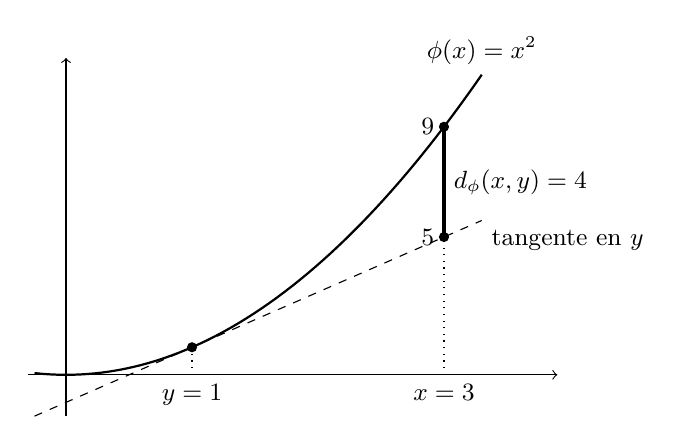
\begin{tikzpicture}[xscale=1.6, yscale=0.35]
    \draw[->] (-0.3,0) -- (3.9,0);
    \draw[->] (0,-1.5) -- (0,11.5);
    \draw[thick, domain=-0.25:3.3, samples=60] plot (\x,{\x*\x})
      node[above] {\small $\phi(x) = x^2$};
    \draw[dashed, domain=-0.25:3.3] plot (\x,{2*\x-1})
      node[below right] {\small tangente en $y$};
    \draw[dotted] (1,0) -- (1,1);
    \draw[dotted] (3,0) -- (3,5);
    \draw[line width=1.6pt] (3,5) -- (3,9);
    \node[right] at (3,7) {\small $d_\phi(x,y) = 4$};
    \node[circle, fill, inner sep=1.3pt] at (1,1) {};
    \node[circle, fill, inner sep=1.3pt] at (3,9) {};
    \node[circle, fill, inner sep=1.3pt] at (3,5) {};
    \node[left] at (3,9) {\small 9};
    \node[left] at (3,5) {\small 5};
    \node[below] at (1,0) {\small $y = 1$};
    \node[below] at (3,0) {\small $x = 3$};
  \end{tikzpicture}
  \caption{Divergencia de Bregman para $\phi(x) = x^2$, con representante
  $y = 1$ y dato $x = 3$. La divergencia es la distancia vertical, en $x$, entre
  la curva y su recta tangente en $y$.}
  \label{fig:bregman}
\end{figure}

En esta tesis los datos no son números sueltos sino matrices, y la recta
tangente se convierte en un plano tangente con una pendiente por cada celda. La
definición general \cite{Bregman1967} considera una función
$\phi : S \subseteq \mathbb{R}^p \to \mathbb{R}$ estrictamente convexa y
diferenciable en el interior relativo de $S$, y define la divergencia de Bregman
asociada a $\phi$ como
\begin{equation}\label{eq:bregman}
  d_\phi(x, y) = \phi(x) - \phi(y) - \langle x - y, \nabla\phi(y) \rangle ,
\end{equation}
donde $\nabla\phi(y)$ es el vector de pendientes de $\phi$ en $y$, una por
componente, y $\langle a, b \rangle = \sum_k a_k b_k$ suma los productos
componente a componente. Con una sola componente, \eqref{eq:bregman} coincide
con~\eqref{eq:bregman-1d}.

De esta construcción se siguen las propiedades que se usan en el resto del
capítulo. La divergencia es no negativa y solo vale cero cuando el dato coincide
con el representante, por lo que puede usarse como función de pérdida. Es además
convexa en su primer argumento. En general no es simétrica,
$d_\phi(x, y) \neq d_\phi(y, x)$, porque la tangente se traza en el
representante y no en el dato, y tampoco cumple la desigualdad triangular. Por
eso no es una métrica, y se la llama divergencia y no distancia. Por último,
cuando $\phi$ es una suma de funciones de cada componente,
$\phi(x) = \sum_k \phi(x_k)$, la divergencia también lo es,
$d_\phi(x, y) = \sum_k d_\phi(x_k, y_k)$. Esta propiedad permite medir la
discrepancia entre dos matrices sumando la discrepancia celda por celda.

La Tabla~\ref{tab:bregman} reúne los tres casos que aparecen en esta tesis, cada
uno obtenido con una función $\phi$ distinta. Cada $\phi$ corresponde a un
supuesto distinto sobre cómo varía el error con la magnitud del dato, de modo que
es constante en la distancia euclídea y proporcional a la media en la
I-divergencia. La I-divergencia, término
introducido por \cite{Csiszar1975} para distribuciones de probabilidad y extendido
por \cite{Csiszar1991} a vectores no negativos que no suman uno, generaliza la
divergencia de Kullback--Leibler a datos como las matrices de conteos. A
diferencia de la distancia euclídea, pesa cada diferencia según la magnitud de la
celda. Una diferencia de 10 viajes vale 0.48 en una celda con 100 y 0.005 en una
con 10\,000, mientras que la distancia euclídea vale 100 en ambos casos. Esa
ponderación es la del modelo de Poisson, y la
Sección~\ref{sec:bregman-expfam} muestra que la correspondencia es exacta. En la
I-divergencia se adopta la convención $0 \log 0 = 0$, de modo que el dato puede
valer cero, mientras que el representante debe ser positivo.

\begin{table}[ht]
  \centering
  {\footnotesize
  \renewcommand{\arraystretch}{1.4}
  \begin{tabular}{@{}lccc@{}}
    \toprule
    \textbf{Divergencia} & \textbf{Dominio} & $\phi(x)$ & $d_\phi(x,y)$ \\
    \midrule
    Euclídea al cuadrado & $\mathbb{R}$ & $x^2$ & $(x-y)^2$ \\
    \midrule
    Kullback--Leibler & símplex & $\sum_k x_k \log x_k$ & $\sum_k x_k \log (x_k/y_k)$ \\
    \midrule
    I-divergencia & $\mathbb{R}_{+}$ & $x \log x - x$ & $x \log (x/y) - (x - y)$ \\
    \bottomrule
  \end{tabular}
  }
  \caption{Divergencias de Bregman utilizadas en esta tesis.}
  \label{tab:bregman}
\end{table}

Cada una de las tres divergencias cumple un papel distinto en la tesis. La
I-divergencia es la que se aplica a los datos, porque la matriz de co-ocurrencia
contiene conteos de viajes y esta divergencia pondera el error según el tamaño
de la celda y coincide con el modelo de Poisson. La divergencia de
Kullback--Leibler es la que conecta con la literatura del co-agrupamiento por
información mutua, ya que la función objetivo declarada por \cite{Liu2021} es la
pérdida de información mutua, que se define con ella
(Sección~\ref{sec:stcc-base}). La distancia euclídea es el caso clásico y sirve
de referencia, ya que permite introducir la intuición, explicar K-means y la
varianza, y comparar con el co-agrupamiento clásico de bloques constantes.

Una propiedad de la I-divergencia que se usará más adelante es su homogeneidad.
Si el dato y el representante se multiplican por una misma constante $c > 0$, la
divergencia queda multiplicada por $c$,
\begin{equation}\label{eq:homogeneidad}
  d_I(cx, cy) = c \, d_I(x, y).
\end{equation}
Esta propiedad implica que multiplicar toda una matriz por una constante
multiplica su divergencia por esa misma constante, sin alterar cuál es la
partición óptima, aspecto que se retoma al distinguir entre conteos y promedios
en la Sección~\ref{sec:escala}.

\subsection{La media como mejor representante}

Cada grupo de datos se resume con un solo representante, y la pregunta es qué
número conviene elegir para que el error promedio sea el menor posible. La
propiedad que justifica el uso de las divergencias de Bregman en agrupamiento
es que, para todas ellas, la respuesta es la media aritmética del grupo
\cite[Prop.~1]{Banerjee2005}.

Sea $X$ un dato del grupo tomado al azar, con media $\mu = \mathrm{E}[X]$, donde
$\mathrm{E}[\cdot]$ denota el promedio sobre todos los datos del grupo. Sea $s$
cualquier número que se proponga como representante. Entonces
\begin{equation}\label{eq:media}
  \mathrm{E}[d_\phi(X, s)] = \mathrm{E}[d_\phi(X, \mu)] + d_\phi(\mu, s).
\end{equation}
Cada parte de la ecuación tiene una lectura directa. El primer miembro,
$\mathrm{E}[d_\phi(X, s)]$, es el error promedio al usar $s$ como representante,
que se obtiene calculando el error de cada dato contra $s$ y promediándolos. El
primer término del segundo miembro, $\mathrm{E}[d_\phi(X, \mu)]$, es el mismo
error promedio cuando el representante es la media. El último término,
$d_\phi(\mu, s)$, no es un promedio sino un único número que indica qué tan lejos
está $s$ de la media. En palabras,
el error de usar cualquier representante es el error de usar la media más un
castigo por haberse alejado de ella.

Como toda divergencia es no negativa y solo se anula cuando sus dos argumentos
coinciden, el castigo es cero únicamente si $s = \mu$. Cualquier otro
representante tiene un error mayor, de modo que la media es el único
representante óptimo. Por ejemplo, sea un grupo con los datos $1$, $2$ y $6$, de
media $\mu = 3$, y sea $\phi(x) = x^2$. Con $s = 3$ el error promedio es
$(4 + 1 + 9)/3 \approx 4.67$. Con $s = 2$ es $(1 + 0 + 16)/3 \approx 5.67$, y la
diferencia es exactamente $d_\phi(3, 2) = (3 - 2)^2 = 1$. La identidad no depende
de $\phi$, ya que con la I-divergencia los valores son distintos, $0.750$ con $s = 3$ y
$0.966$ con $s = 2$, pero la diferencia sigue siendo $d_I(3, 2) \approx 0.216$.

En consecuencia, un algoritmo de tipo K-means que calcula centroides como medias
es válido para cualquier divergencia de Bregman, no solo para la euclídea, porque
en el paso en que se recalcula cada representante, la media es siempre la mejor
elección.
\cite{Banerjee2005opt} demostraron además el recíproco, a saber, que bajo condiciones de
regularidad suaves sobre la función de pérdida, las divergencias de Bregman son
las únicas para las que la media condicional es el predictor óptimo
\cite[Teoremas~3 y~4]{Banerjee2005opt}.

El valor mínimo de~\eqref{eq:media} recibe el nombre de información de
Bregman de $X$ y se escribe
\begin{equation}\label{eq:info-bregman}
  I_\phi(X) = \mathrm{E}[d_\phi(X, \mathrm{E}[X])].
\end{equation}
Es el error que queda al usar el mejor representante, la media, y mide cuánta
variabilidad del grupo no puede capturar un único representante. Si todos los
datos son iguales, la media los representa sin error y $I_\phi(X) = 0$; cuanto
más dispersos están, mayor es.

Con la distancia euclídea, $I_\phi(X)$ es la varianza de $X$. En el ejemplo
anterior, con los datos $1$, $2$ y $6$, vale $(4 + 1 + 9)/3 \approx 4.67$, que es
el promedio de los desvíos al cuadrado respecto de la media. Con la divergencia
de Kullback--Leibler, que compara dos distribuciones de probabilidad y vale cero
solo cuando coinciden, los datos son distribuciones. Si $X$ toma como valores las
distribuciones condicionales $p(Y \mid U = u)$ con probabilidad $p(u)$, su media
es la distribución marginal $p(Y)$ y la información de Bregman es la
información mutua $I(U;Y)$ \cite{Banerjee2005}. Es decir, mide cuánto se parece
cada distribución condicional a la marginal, de modo que si todas coinciden con
ella, saber $U$ no dice nada sobre $Y$ y la información mutua es cero. Esta
doble lectura explica por qué
un mismo marco puede generalizar tanto el agrupamiento por mínima varianza como el
co-agrupamiento que minimiza la pérdida de información mutua.

\subsection{Relación con las familias exponenciales}\label{sec:bregman-expfam}

Hasta aquí se ha justificado la I-divergencia por sentido común, porque pesa cada
diferencia según el tamaño de la celda. Esta sección muestra que corresponde
exactamente a un modelo estadístico, lo que permite leer el método como el ajuste
de un modelo y no solo como una regla de pérdida. Esta lectura es importante para
la tesis porque, una vez que el co-agrupamiento se interpreta como el ajuste de
un modelo de Poisson, es posible someter sus resultados a pruebas de hipótesis y
cuantificar si la estructura que se encuentra en un bloque es real o es solo
ruido de los datos.

Una familia exponencial es una colección de distribuciones, como la normal, la
Poisson o la binomial, que comparten una misma forma matemática y que tienen un
parámetro de media $\mu$. \cite{Banerjee2005} establecieron una correspondencia
uno a uno entre las divergencias de Bregman regulares y las familias
exponenciales regulares \cite[Teoremas~4 y~6]{Banerjee2005}, de modo que la
densidad de cada familia puede escribirse como
\begin{equation}\label{eq:expfam}
  p(x \mid \mu) = \exp\{-d_\phi(x, \mu)\}\, b_\phi(x),
\end{equation}
donde $\mu$ es el parámetro de media y $b_\phi$ depende solo del dato, no de
$\mu$. La lectura es directa, pues un dato es más probable cuanto más cerca está de la
media, y la cercanía se mide con la divergencia de Bregman de esa familia. La
distancia euclídea corresponde, salvo un factor de escala, a la normal con
varianza fija $\sigma^2$, cuya divergencia es
$\lVert x - \mu \rVert^2 / (2\sigma^2)$; la I-divergencia corresponde a la
distribución de Poisson. Es la misma idea de la Tabla~\ref{tab:bregman}, con un
supuesto estadístico concreto detrás de cada $\phi$.

Para el caso de Poisson la correspondencia puede verificarse directamente. Si
$x \sim \mathrm{Poisson}(\mu)$, su log-verosimilitud es
$x \log \mu - \mu - \log x!$, y
\begin{equation}\label{eq:poisson-idiv}
  \log p(x \mid \mu) = -d_I(x, \mu) + \underbrace{\left( x \log x - x - \log x! \right)}_{\text{no depende de } \mu}.
\end{equation}
Por ejemplo, con $x = 4$ y $\mu = 3$ la probabilidad es $0.168$, de modo que
$\log p = -1.784$. La I-divergencia vale $d_I(4, 3) = 0.151$ y el término que no
depende de $\mu$ vale $-1.633$, y $-0.151 - 1.633 = -1.784$. Como ese último
término no depende de $\mu$, al comparar medias candidatas solo importa
$-d_I(x, \mu)$, y por tanto la media con menor divergencia es la de mayor verosimilitud. Con
$x = 4$, la media $\mu = 5$ tiene divergencia $0.107$ y $\log p = -1.740$,
mejor en ambos sentidos que $\mu = 3$, con $0.151$ y $-1.784$.

Para una matriz de conteos independientes $O_{ij} \sim
\mathrm{Poisson}(\mu_{ij})$, como la I-divergencia es aditiva por celda,
\begin{equation}\label{eq:devianza}
  D_I(O \,\|\, \mu) \;=\; \sum_{i,j} d_I(O_{ij}, \mu_{ij}) \;=\; \tfrac{1}{2}\, \mathrm{Dev}(\mu),
\end{equation}
donde $\mathrm{Dev}(\mu) = 2 \sum_{i,j} [\, O_{ij} \log (O_{ij}/\mu_{ij}) - (O_{ij} - \mu_{ij}) \,]$
es la devianza del modelo de Poisson con medias $\mu$
\cite[Sec.~4.5.2, ec.~4.34]{Agresti2013}, la medida habitual de qué tan mal ajusta
un modelo a los conteos. Aquí $\mu_{ij}$ es lo que predice el modelo para cada
celda, que en esta tesis es la media del bloque al que pertenece. Minimizar la
I-divergencia equivale entonces a maximizar la verosimilitud de Poisson, es decir,
a elegir el modelo de Poisson por bloques que mejor explica los datos. Esta
equivalencia es la que permite, en la Sección~\ref{sec:idiv-poisson}, leer el
co-agrupamiento como el ajuste de un modelo estadístico.

% ---------------------------------------------------------------------
\section{Co-agrupamiento de Bregman}\label{sec:bbac}

Las secciones anteriores presentaron dos piezas por separado, las divergencias de
Bregman, que miden el error al reemplazar un dato por un representante, y el
co-agrupamiento, que forma un tablero de bloques. Falta unirlas, es decir, definir
cómo se reconstruye la matriz a partir de los bloques y cómo se mide qué tan
buena es esa reconstrucción. \cite{Banerjee2007} formularon el co-agrupamiento
como un problema de aproximación de matrices en el que la función de pérdida
puede ser cualquier divergencia de Bregman, de modo que se resume la matriz con
unos pocos promedios, se reconstruye una matriz aproximada a partir de ellos y se
eligen los grupos que hacen mínimo el error de esa aproximación. Esta sección
presenta esa formulación con la notación de la tesis.

\subsection{Notación}

Sea $O \in \mathbb{R}_{+}^{m \times n}$ la matriz de co-ocurrencia, con filas
asociadas a regiones y columnas a intervalos de tiempo. Un co-agrupamiento es un
par de funciones
\[
  \rho : \{1, \dots, m\} \to \{1, \dots, K_R\}, \qquad
  \tau : \{1, \dots, n\} \to \{1, \dots, K_T\},
\]
que asignan cada fila a un grupo de filas y cada columna a un grupo de columnas.
Se denota $I_g = \rho^{-1}(g)$ al conjunto de filas del grupo $g$,
$J_h = \tau^{-1}(h)$ al conjunto de columnas del grupo $h$, y
$B_{gh} = I_g \times J_h$ al bloque que forman. Por ejemplo, en una matriz de
cuatro regiones por cuatro intervalos con $\rho$ que agrupa las regiones de dos
en dos y $\tau$ los intervalos de dos en dos, resulta un tablero de
$2 \times 2$ bloques de cuatro celdas cada uno.

Para expresar los promedios de forma compacta, \cite{Banerjee2007} adoptan una
lectura probabilística de la matriz, en la que se elige una celda al azar, con $U$ uniforme
sobre las filas y $V$ uniforme sobre las columnas, y se define la variable
aleatoria $Z = O_{UV}$, el valor de esa celda. Los índices de grupo son
$\hat{U} = \rho(U)$ y $\hat{V} = \tau(V)$. Esta notación permite escribir cada
promedio como una esperanza condicional, es decir, como el promedio de las celdas
que cumplen una condición. Así, $\mathrm{E}[Z]$ es el promedio de toda la matriz,
$\mathrm{E}[Z \mid U = i]$ es la media de la fila $i$ y
$\mathrm{E}[Z \mid \hat{U} = g, \hat{V} = h]$ es la media del bloque $B_{gh}$.

\subsection{Aproximación y principio de mínima información de Bregman}

Un co-agrupamiento resume la matriz mediante un conjunto de promedios. La pregunta
es cuáles promedios conservar y cómo reconstruir la matriz a partir de ellos.
\cite{Banerjee2007} responden con dos elementos. El primero es una base
$\mathcal{C} = \{G_1, \dots, G_s\}$, que indica qué
promedios debe conservar la aproximación. Formalmente es una colección de
conjuntos de variables, cada uno tomado de $\{U, V, \hat{U}, \hat{V}\}$, y la
aproximación conserva las medias condicionales $\mathrm{E}[Z \mid G]$, para
$G \in \mathcal{C}$. La base más simple, $\{\hat{U}, \hat{V}\}$, conserva la media
de cada bloque; la base $\{\hat{U}\}, \{\hat{V}\}$ conserva solo la media de cada
grupo de filas y la de cada grupo de columnas.

El segundo es el principio de mínima información de Bregman (MBI). Con los
promedios fijados hay muchas matrices que los respetan, y el principio elige,
entre todas ellas, la de menor información de Bregman~\eqref{eq:info-bregman}.
Como esa información mide la variabilidad, se elige la matriz más simple
compatible con los promedios, pues la idea es no añadir a la aproximación más
estructura que la exigida por los estadísticos. Con la
I-divergencia o la divergencia de Kullback--Leibler, este principio coincide con el
de máxima entropía. Los autores demuestran que la solución MBI, denotada
$\hat{Z}_{\mathcal{C}}$, es también la mejor aproximación, en divergencia esperada,
entre las que tienen su misma forma funcional, y que satisface una propiedad
pitagórica \cite[Lema~3 y Teorema~2]{Banerjee2007} que se usará en la
Sección~\ref{sec:descomposicion}.

Fijadas la divergencia $\phi$ y la base $\mathcal{C}$, el co-agrupamiento de
Bregman busca
\begin{equation}\label{eq:objetivo-bregman}
  (\rho^*, \tau^*) = \operatorname*{arg\,min}_{\rho,\, \tau}\;
  \mathrm{E}\!\left[ d_\phi\!\left(Z, \hat{Z}_{\mathcal{C}}(\rho, \tau)\right) \right],
\end{equation}
que, con medida uniforme sobre las celdas, es proporcional a
$\sum_{i,j} d_\phi(O_{ij}, \hat{O}_{ij})$. Es decir, entre todos los
co-agrupamientos posibles se elige el que hace mínimo el error entre la matriz
real y su aproximación.

Un ejemplo ayuda a ver el efecto de la base. Sea la matriz de cuatro regiones por
cuatro intervalos
\[
  O = \begin{pmatrix}
    12 & 8 & 3 & 1 \\
    8 & 12 & 1 & 3 \\
    2 & 2 & 10 & 6 \\
    2 & 2 & 6 & 10
  \end{pmatrix},
\]
con las regiones y los intervalos agrupados de dos en dos, de modo que las medias
de los cuatro bloques son $10$, $2$, $2$ y $8$. Con la base $\{\hat{U}, \hat{V}\}$
la matriz más simple compatible con esas medias rellena cada bloque con la suya, y
la I-divergencia entre $O$ y esa aproximación suma $2.86$. Con la base
$\{\hat{U}\}, \{\hat{V}\}$, en cambio, las medias por grupo de filas son $6$ y $5$,
las de columnas son $6$ y $5$, la media global es $5.5$ y la aproximación con
I-divergencia es el producto $\mathrm{E}[Z|\hat{U}]\,\mathrm{E}[Z|\hat{V}] /
\mathrm{E}[Z]$, que da $6.55$, $5.45$, $5.45$ y $4.55$ en los cuatro bloques. Esa
aproximación respeta las medias por grupo, pero no distingue que el primer bloque
es mucho más alto que el segundo. La base determina así qué estructura puede
capturar la aproximación.

\subsection{Las seis bases}\label{sec:bases}

Cada base responde a la pregunta de cuánto detalle se quiere conservar además de
dividir la matriz en bloques. \cite[Teorema~3]{Banerjee2007} muestran que en dos
dimensiones existen seis bases no triviales y no redundantes, es decir, que
resumen la matriz y que ninguna produce la misma aproximación que otra. La
Tabla~\ref{tab:bases} las resume junto con la forma cerrada de la aproximación
cuando se usa la I-divergencia, que se obtiene como producto y cociente de las
medias condicionales conservadas. En la tabla, $U$ y $V$ designan una fila y una
columna individuales, y $\hat{U}$ y $\hat{V}$ sus grupos; un conjunto como
$\{\hat{U}, \hat{V}\}$ conserva la media de cada bloque y $\{U\}$ la de cada fila.

\begin{table}[ht]
  \centering
  {\footnotesize
  \renewcommand{\arraystretch}{1.4}
  \begin{tabular}{@{}l p{0.18\textwidth} p{0.30\textwidth} p{0.32\textwidth}@{}}
    \toprule
    \textbf{Base} & \textbf{Conjuntos} & \textbf{Medias que conserva} & \textbf{Aproximación con $d_I$} \\
    \midrule
    C1 & $\{\hat{U}\}, \{\hat{V}\}$ & de cada grupo de filas y de cada grupo de columnas &
      $\mathrm{E}[Z|\hat{U}]\,\mathrm{E}[Z|\hat{V}] \,/\, \mathrm{E}[Z]$ \\
    \midrule
    C2 & $\{\hat{U}, \hat{V}\}$ & de cada bloque &
      $\mathrm{E}[Z|\hat{U},\hat{V}]$ \\
    \midrule
    C3 & $\{\hat{U}, \hat{V}\}, \{U\}$ & de cada bloque y de cada fila &
      $\mathrm{E}[Z|U]\,\mathrm{E}[Z|\hat{U},\hat{V}] \,/\, \mathrm{E}[Z|\hat{U}]$ \\
    \midrule
    C4 & $\{\hat{U}, \hat{V}\}, \{V\}$ & de cada bloque y de cada columna &
      $\mathrm{E}[Z|V]\,\mathrm{E}[Z|\hat{U},\hat{V}] \,/\, \mathrm{E}[Z|\hat{V}]$ \\
    \midrule
    C5 & $\{\hat{U}, \hat{V}\}, \{U\}, \{V\}$ & de cada bloque, fila y columna &
      $\dfrac{\mathrm{E}[Z|U]\,\mathrm{E}[Z|V]\,\mathrm{E}[Z|\hat{U},\hat{V}]}{\mathrm{E}[Z|\hat{U}]\,\mathrm{E}[Z|\hat{V}]}$ \\
    \midrule
    C6 & $\{U, \hat{V}\}, \{\hat{U}, V\}$ & de cada fila dentro de cada grupo de columnas, y de cada columna dentro de cada grupo de filas &
      $\mathrm{E}[Z|U,\hat{V}]\,\mathrm{E}[Z|\hat{U},V] \,/\, \mathrm{E}[Z|\hat{U},\hat{V}]$ \\
    \bottomrule
  \end{tabular}
  }
  \caption{Bases de co-agrupamiento de Bregman en dos dimensiones
  \cite{Banerjee2007} y forma de la aproximación con I-divergencia, bajo medida
  uniforme sobre las celdas.}
  \label{tab:bases}
\end{table}

La forma de la base C5 es la más fácil de leer. Reagrupada, la aproximación es la
media del bloque multiplicada por dos factores,
\[
  \hat{O}_{ij} = \mathrm{E}[Z|\hat{U},\hat{V}] \cdot
  \frac{\mathrm{E}[Z|U]}{\mathrm{E}[Z|\hat{U}]} \cdot
  \frac{\mathrm{E}[Z|V]}{\mathrm{E}[Z|\hat{V}]},
\]
donde cada factor compara una fila, o una columna, con su grupo, de modo que si
una región tiene el doble de viajes que el promedio de su grupo, su factor es 2. Las bases C3
y C4 aplican solo el factor de fila o el de columna, respectivamente, y C2 no
aplica ninguno. Así, C5 distingue entre una región que es más grande y una que
tiene un patrón distinto. Un ejemplo mínimo lo muestra. Sea la matriz de un solo
bloque
\[
  \begin{pmatrix} 2 & 4 \\ 6 & 12 \end{pmatrix},
\]
cuya segunda fila tiene el triple de viajes que la primera con el mismo perfil.
Las medias de fila son $3$ y $9$, las de columna $4$ y $8$, y la global $6$. Con
la base C2 todas las celdas valen $6$ y la I-divergencia suma $4.50$. Con la base
C5 la aproximación es $\mathrm{E}[Z|U]\,\mathrm{E}[Z|V]/\mathrm{E}[Z]$, que
reproduce la matriz exacta y da pérdida cero, porque C5 descuenta el volumen de cada fila
y de cada columna, que es la diferencia que motiva su elección en esta tesis
(Sección~\ref{sec:stcc-base}).

Varios métodos conocidos resultan ser casos particulares de este esquema. La base
C2 con distancia euclídea es el co-agrupamiento clásico de bloques constantes, que
corresponde al primer residuo de \cite{Cho2004}. La base C6 con distancia euclídea
es el co-agrupamiento por residuo cuadrático mínimo de \cite{Cho2004}, que usa el
segundo residuo, $O_{ij} - \mathrm{E}[Z|U,\hat{V}] - \mathrm{E}[Z|\hat{U},V] +
\mathrm{E}[Z|\hat{U},\hat{V}]$ \cite[Ejemplo~2.F]{Banerjee2007}; sobre él se
construye el BCC\_MSSR de \cite{Wu2022}. La base C5 con I-divergencia, que sobre
una distribución conjunta coincide con la divergencia de Kullback--Leibler, es el
co-agrupamiento de teoría de la información (ITCC) de \cite{Dhillon2003}, que
minimiza la pérdida de información mutua entre filas y columnas
\cite[Ejemplo~1.F]{Banerjee2007}.

Cabe notar que la base C6 aparece en los dos contextos de este capítulo. Con
distancia euclídea combina las marginales internas del bloque de forma aditiva,
como en el residuo de \cite{Cho2004}, y con I-divergencia las combina de forma
multiplicativa, como en la prueba de independencia dentro del bloque que se usa
en la Sección~\ref{sec:idiv-poisson}. Es la misma estructura con dos álgebras, ya que la
euclídea trabaja con diferencias y la I-divergencia con razones.

\subsection{Algoritmo}\label{sec:bbac-algoritmo}

Falta decir cómo se encuentra la partición que hace mínimo el
problema~\eqref{eq:objetivo-bregman}. Probar todas las particiones es inviable, ya que solo
asignar 100 filas a 5 grupos admite del orden de $5^{100} \approx 10^{70}$
posibilidades, sin contar las columnas. El problema es combinatorio y de hecho
NP-difícil por reducción desde el problema de K-means \cite{Banerjee2007}, es
decir, no se conoce un método eficiente que garantice la mejor partición. Por eso
\cite{Banerjee2007} proponen un algoritmo de minimización alternante, con la misma
idea que K-means, en el que con los grupos fijos se calculan los mejores promedios y con los
promedios fijos se mejoran los grupos. Sus pasos son los siguientes.

\begin{enumerate}
  \item Inicializar $\rho$ y $\tau$, por ejemplo al azar.
  \item Calcular los estadísticos de la base y la aproximación $\hat{O}$.
  \item Con $\tau$ y los estadísticos fijos, reasignar cada fila al grupo que
        mejor la explica. Formalmente, la fila $i$ pasa al grupo $g$ que minimiza
        su contribución a la divergencia, $\sum_j d_\phi(O_{ij}, \hat{O}_{ij})$,
        calculada como si $i$ perteneciera a $g$. Recalcular los estadísticos.
  \item Repetir el paso anterior para las columnas, con $\rho$ fija.
  \item Si la reducción de la divergencia es menor que un umbral $\varepsilon$,
        terminar; si no, volver al paso 3.
\end{enumerate}

Un ejemplo con la matriz de cuatro regiones por cuatro intervalos de la
Sección~\ref{sec:bbac}, base C2 e I-divergencia, muestra el paso 3. Si $\tau$ es
la correcta y $\rho$ empieza mal, con las regiones $r_1, r_2, r_3$ en un grupo y
$r_4$ en otro, el error total es $15.6$. Para la fila $r_3 = (2, 2, 10, 6)$, el
error de quedarse con $r_1$ y $r_2$ es $9.07$, porque se la compara con las medias
$(7.33, 7.33, 4, 4)$, y el de pasar al grupo de $r_4$ es $0.51$, porque se la
compara con $(2, 2, 8, 8)$. La fila cambia de grupo, la partición de filas queda
correcta y el error baja a $2.86$.

Cada paso no aumenta el valor de la función objetivo, porque al recalcular los
estadísticos, la media es el mejor representante de cada grupo
(Sección~\ref{sec:bregman}), y al reasignar, cada fila elige el grupo que menos
error le produce. Como además el número de particiones es finito, el algoritmo
converge en un número finito de iteraciones. Sin embargo, converge a un mínimo
local, es decir, una solución que no mejora cambiando el agrupamiento de filas, el de
columnas o los estadísticos de la base \cite[Teorema~6]{Banerjee2007}. Es como
bajar una montaña por el camino más empinado, que lleva a un valle pero no
necesariamente al más profundo. Esta optimalidad es relativa a las
actualizaciones por lotes; \cite{Cho2004} muestran que una búsqueda local que
mueve filas o columnas de una en una puede seguir reduciendo el objetivo después
de la convergencia. Por eso se ejecuta con varias inicializaciones y se conserva
la mejor solución, y cada ejecución puede completarse con esa búsqueda local;
\cite{Liu2021}, por ejemplo, usaron 200 inicializaciones. Para una matriz densa,
cada iteración cuesta $O\!\left(mn(K_R + K_T)\right)$ operaciones
\cite[Sec.~4.4]{Cho2004}.

% ---------------------------------------------------------------------
\section{El caso de la I-divergencia y su lectura como modelo de Poisson}\label{sec:idiv-poisson}

Esta sección particulariza el marco anterior a la I-divergencia y a matrices de
conteos, que es el caso de ST-CC y de esta tesis. Se mostrará que cada base
corresponde a un modelo de Poisson, que tres de esas bases forman una cadena de
modelos anidados, y que la divergencia de ST-CC se descompone en términos con
interpretación propia. Esto permite interpretar los resultados como el ajuste de
un modelo estadístico y justifica el estadístico de heterogeneidad del método
propuesto, pues el marco anterior funciona con cualquier divergencia, pero esta tesis
usa una sola, con conteos de viajes, y es en ese caso donde aparecen estas
propiedades.

\subsection{Tres bases en notación matricial}

Además de los totales de fila $O_{i\cdot} = \sum_j O_{ij}$, de columna
$O_{\cdot j} = \sum_i O_{ij}$ y general $N$, se usan los totales por grupo y por
bloque, definidos como
\[
  O_{g\cdot} = \sum_{i \in I_g} O_{i\cdot}, \qquad
  O_{\cdot h} = \sum_{j \in J_h} O_{\cdot j}, \qquad
  N_{gh} = \sum_{(i,j) \in B_{gh}} O_{ij},
\]
y las marginales dentro de un bloque, definidas como
\[
  O_{ih} = \sum_{j \in J_h} O_{ij} \quad (i \in I_g), \qquad
  O_{gj} = \sum_{i \in I_g} O_{ij} \quad (j \in J_h).
\]
Es decir, $O_{ih}$ es el total de la fila $i$ dentro del grupo de columnas $h$, y
$O_{gj}$ el total de la columna $j$ dentro del grupo de filas $g$. Son los mismos
promedios de la sección anterior escritos como sumas. En una matriz de cuatro
regiones por cuatro intervalos agrupados de dos en dos, con las filas de
totales $24$, $24$, $20$ y $20$, por ejemplo, $O_{1\cdot} = 24$ y $N = 88$.

Al traducir la Tabla~\ref{tab:bases} a esta notación, para una celda
$(i,j) \in B_{gh}$ las tres bases relevantes toman la forma
\begin{align}
  \hat{O}^{\mathrm{C2}}_{ij} &= \frac{N_{gh}}{|I_g|\,|J_h|}, \label{eq:c2}\\[4pt]
  \hat{O}^{\mathrm{C5}}_{ij} &= \frac{O_{i\cdot}\; O_{\cdot j}\; N_{gh}}{O_{g\cdot}\; O_{\cdot h}}, \label{eq:c5}\\[4pt]
  \hat{O}^{\mathrm{C6}}_{ij} &= \frac{O_{ih}\; O_{gj}}{N_{gh}}. \label{eq:c6}
\end{align}

La base C2 asigna a todas las celdas del bloque el mismo valor, que es su media. La base
C5 reparte el total del bloque en proporción al volumen global de cada región y de
cada intervalo, de modo que una región con mucha actividad recibe más viajes en
todos los bloques de su fila; es la media del bloque escalada por los factores de
fila y de columna de la Sección~\ref{sec:bases}. Esta aproximación coincide, salvo el factor $N$, con
la distribución $q(r,t)$ de \cite{Dhillon2003}, y su divergencia es la pérdida de información
mutua,
\begin{equation}\label{eq:perdida-im}
  D_I\!\left(O \,\|\, \hat{O}^{\mathrm{C5}}\right) = N \left[ I(R;T) - I(\hat{R};\hat{T}) \right],
\end{equation}
donde las informaciones mutuas se calculan sobre la distribución empírica $O/N$ y
su versión agregada por bloques.

La base C6 trata cada bloque como una tabla de contingencia independiente y la
aproxima por el producto de sus propias marginales, es decir, por los conteos
esperados bajo independencia entre filas y columnas dentro del bloque. Su
divergencia se descompone por bloques,
\begin{equation}\label{eq:c6-g2}
  D_I\!\left(O \,\|\, \hat{O}^{\mathrm{C6}}\right)
  = \tfrac{1}{2} \sum_{g,h} G^2_{gh}, \qquad
  G^2_{gh} = 2 \sum_{(i,j) \in B_{gh}} O_{ij} \log \frac{O_{ij}\, N_{gh}}{O_{ih}\, O_{gj}},
\end{equation}
donde $G^2_{gh}$ es el estadístico de razón de verosimilitud de la prueba de
independencia en la tabla $O|_{B_{gh}}$ \cite[Sec.~3.2.1, ec.~3.11]{Agresti2013}.
Este estadístico también puede escribirse como
\begin{equation}\label{eq:g2-im}
  G^2_{gh} = 2\, N_{gh}\, \hat{I}_{gh}(R;T),
\end{equation}
donde $\hat{I}_{gh}(R;T)$ es la información mutua de la distribución empírica del
bloque, $O_{ij}/N_{gh}$ para $(i,j) \in B_{gh}$. Es decir, $G^2_{gh}$ mide cuánta
asociación entre regiones y horarios queda dentro del bloque, escalada por su masa.
Por ejemplo, en el bloque
$\begin{pmatrix} 6 & 2 \\ 2 & 6 \end{pmatrix}$ los totales de fila y de columna
valen $8$ y $N_{gh} = 16$, de modo que bajo independencia cada celda valdría
$8 \cdot 8 / 16 = 4$. Los datos, en cambio, concentran los viajes en la diagonal, y
resulta $G^2_{gh} = 2\,[\,12 \ln 1.5 + 4 \ln 0.5\,] \approx 4.19$; un bloque con
las cuatro celdas iguales daría $G^2_{gh} = 0$.

\subsection{Equivalencia con modelos log-lineales de Poisson}\label{sec:loglineal}

Por la equivalencia~\eqref{eq:devianza}, minimizar $D_I(O \,\|\, \hat{O})$ equivale a
maximizar una verosimilitud de Poisson. Cada base define, además, un modelo
log-lineal concreto para las medias $\mu_{ij}$, a saber,
\begin{align}
  \text{C2:}\quad & \log \mu_{ij} = \lambda_{\rho(i)\tau(j)}, \label{eq:ll-c2}\\
  \text{C5:}\quad & \log \mu_{ij} = \alpha_i + \beta_j + \lambda_{\rho(i)\tau(j)}, \label{eq:ll-c5}\\
  \text{C6:}\quad & \log \mu_{ij} = \alpha_{i,\tau(j)} + \beta_{\rho(i),j}. \label{eq:ll-c6}
\end{align}
En C2 hay un nivel por bloque. En C5 se añaden efectos globales de fila y de
columna. En C6 el efecto de cada fila puede cambiar según el grupo de columnas y
el efecto de cada columna según el grupo de filas. Un modelo log-lineal suma
efectos en el logaritmo, de modo que al deshacerlo los efectos se multiplican y C5
es la media del bloque por un factor de fila y por un factor de columna, la misma
forma de la Sección~\ref{sec:bases}.

Las aproximaciones~\eqref{eq:c2}--\eqref{eq:c6} son los estimadores de máxima
verosimilitud de estos modelos. En efecto, en un modelo log-lineal de Poisson las
ecuaciones de verosimilitud exigen que las medias ajustadas reproduzcan los
totales observados asociados a cada término del modelo
\cite[Secs.~4.4.9 y~9.6.2]{Agresti2013}, y esos totales son justamente las medias
que conserva cada base. Por otro lado, el logaritmo de cada aproximación tiene la
forma aditiva del modelo correspondiente. El resultado de Birch garantiza que existe un
único conjunto de valores ajustados que satisface el modelo y reproduce los
estadísticos suficientes, y ese conjunto es la solución de máxima verosimilitud
\cite[Sec.~9.6.3]{Agresti2013}; la unicidad se sigue también de que la
verosimilitud de Poisson es cóncava en $\log \mu$.

Para una partición $(\rho, \tau)$ fija, los tres modelos están anidados, es decir,
$\mathrm{C2} \subset \mathrm{C5} \subset \mathrm{C6}$. La primera inclusión se
obtiene con $\alpha = \beta = 0$. La segunda, reescribiendo el modelo C5 como
$\alpha_{i,h} = \alpha_i + \lambda_{\rho(i) h}$ y $\beta_{g,j} = \beta_j$. El
número de parámetros libres de cada modelo se muestra en la
Tabla~\ref{tab:parametros}. En la matriz de cuatro regiones por cuatro intervalos
con $K_R = K_T = 2$, los tres modelos tienen $4$, $8$ y $12$ parámetros, frente a
$16$ del modelo saturado. A más parámetros el modelo es más flexible y el error
menor, pero crece el riesgo de ajustar el ruido.

\begin{table}[ht]
  \centering
  {\footnotesize
  \renewcommand{\arraystretch}{1.4}
  \begin{tabular}{@{}lc@{}}
    \toprule
    \textbf{Modelo} & \textbf{Parámetros libres} \\
    \midrule
    C2 & $K_R K_T$ \\
    C5 & $K_R K_T + (m - K_R) + (n - K_T)$ \\
    C6 & $K_T\, m + K_R\, n - K_R K_T$ \\
    Saturado & $m\,n$ \\
    \bottomrule
  \end{tabular}
  }
  \caption{Número de parámetros de los modelos log-lineales asociados a las bases
  C2, C5 y C6 para una partición fija.}
  \label{tab:parametros}
\end{table}

La diferencia entre el modelo saturado y C6 es
$\sum_{g,h} (|I_g| - 1)(|J_h| - 1)$, que coincide con la suma de los grados de
libertad de las pruebas de independencia en cada bloque. Esto significa que lo
que C6 deja sin explicar respecto del modelo saturado es precisamente la
asociación interna de cada bloque, que es la que miden los estadísticos
$G^2_{gh}$ y la que el método propuesto busca refinar.

\subsection{Descomposición de la divergencia}\label{sec:descomposicion}

Cuando una partición deja un error grande, interesa saber de qué está hecho ese
error. La cadena de modelos anidados permite descomponer la divergencia que deja
una partición de tipo C2 en tres partes. La descomposición se apoya en la
propiedad pitagórica de la I-divergencia \cite{Csiszar1975} y de las soluciones
MBI \cite[Lema~3]{Banerjee2007}, que dice, en palabras, que el error del modelo
simple es el error del modelo complejo más la distancia entre ambos, la misma
estructura de la identidad~\eqref{eq:media}.

\begin{proposicion}[Descomposición de la divergencia]\label{prop:descomposicion}
Sea $(\rho,\tau)$ una partición fija y supóngase que todas las aproximaciones son
positivas en las celdas donde $O_{ij} > 0$. Entonces
\begin{equation}\label{eq:descomposicion}
  D_I\!\left(O \,\|\, \hat{O}^{\mathrm{C2}}\right)
  = \underbrace{D_I\!\left(\hat{O}^{\mathrm{C5}} \,\|\, \hat{O}^{\mathrm{C2}}\right)}_{\text{(i) efectos marginales}}
  + \underbrace{D_I\!\left(\hat{O}^{\mathrm{C6}} \,\|\, \hat{O}^{\mathrm{C5}}\right)}_{\text{(ii) marginales por bloque}}
  + \underbrace{\tfrac{1}{2} \textstyle\sum_{g,h} G^2_{gh}}_{\text{(iii) interacción local}} .
\end{equation}
\end{proposicion}

\begin{proof}
Sean $\mu^s$ y $\mu^b$ los estimadores de máxima
verosimilitud de dos modelos log-lineales anidados $M_s \subset M_b$. Por
definición de la I-divergencia,
\[
  D_I(O \,\|\, \mu^s) - D_I(O \,\|\, \mu^b)
  = \sum_{i,j} O_{ij} \log \frac{\mu^b_{ij}}{\mu^s_{ij}}
  + \sum_{i,j} \mu^s_{ij} - \sum_{i,j} \mu^b_{ij}.
\]
Tanto $\log \mu^s$ como $\log \mu^b$ pertenecen al espacio lineal generado por los
términos de $M_b$, y $\mu^b$ reproduce los totales observados de todos esos
términos. Por lo tanto, el primer sumando puede escribirse con $\mu^b_{ij}$ en
lugar de $O_{ij}$, y la expresión se convierte en $D_I(\mu^b \,\|\, \mu^s)$. Se
obtiene así
$D_I(O \,\|\, \mu^s) = D_I(O \,\|\, \mu^b) + D_I(\mu^b \,\|\, \mu^s)$. Al aplicar
esta identidad a los pares $(\mathrm{C2}, \mathrm{C5})$ y
$(\mathrm{C5}, \mathrm{C6})$ y sustituir~\eqref{eq:c6-g2} en el último término se
obtiene~\eqref{eq:descomposicion}.
\end{proof}

La identidad usada en la demostración es un caso particular de los resultados
citados, ya que cada par de modelos cumple las hipótesis del Lema~3 de
\cite{Banerjee2007}, y para aplicar el resultado de \cite{Csiszar1975}, que trabaja
con distribuciones de probabilidad, basta dividir entre $N$ por la
homogeneidad~\eqref{eq:homogeneidad}. Con esta identidad, cada término de la
descomposición queda asociado a una pregunta distinta sobre los datos, como se
detalla a continuación.

\begin{itemize}
  \item El término (i) mide cuánto de la heterogeneidad dentro de los bloques se
        explica solo porque unas regiones y unos intervalos tienen más volumen
        que otros. Por ejemplo, una zona de Midtown genera más viajes que una del
        norte de Manhattan a cualquier hora. Esto no es interacción
        espacio-temporal.
  \item El término (ii) mide cuánto cambia el peso relativo de una región según el
        grupo de horarios, o el de un intervalo según el grupo de regiones, más
        allá de sus volúmenes globales. Por ejemplo, una región que pesa más en
        los horarios de oficina que en los nocturnos, aunque su volumen total sea
        el mismo.
  \item El término (iii) mide la asociación que queda dentro de cada bloque cuando
        ya se tienen en cuenta sus propias marginales, como ocurre cuando un
        subconjunto de regiones se activa en un subconjunto de horarios del
        bloque de forma distinta al resto. Este es el tipo de patrón local que
        busca esta tesis.
\end{itemize}

La descomposición justifica la elección del estadístico de heterogeneidad del
método propuesto. Si la pregunta es si un bloque contiene un patrón local, el
estadístico adecuado es $G^2_{gh}$, que aísla el término (iii). Un criterio basado
en la constancia del bloque, como el implícito en C2, mezclaría los tres términos
y, en datos de movilidad con volúmenes muy desiguales, detectaría heterogeneidad
en casi todos los bloques solo por el término (i).

Dos ejemplos aíslan los términos. La matriz de un solo bloque
$\begin{pmatrix} 2 & 4 \\ 6 & 12 \end{pmatrix}$ tiene un error de $4.50$ con C2,
pero C5 la reproduce exacta y, con un solo bloque, C6 coincide con C5 y
$G^2 = 0$, de modo que el error es todo del término (i). Parece heterogénea para un criterio
basado en C2, pero es un único perfil multiplicado por el volumen de cada fila y
de cada columna. En cambio, la matriz de cuatro regiones por cuatro intervalos de
la Sección~\ref{sec:bbac} tiene $G^2_{gh}$ de $1.61$, $2.09$, $0$ y $2.02$ en sus
cuatro bloques, de modo que $\tfrac12 \sum G^2_{gh} = 2.86$, que es todo su error
con C2, de modo que los términos (i) y (ii) son nulos y la heterogeneidad es
toda interacción local.

Conviene adelantar una advertencia que se desarrolla en la
Sección~\ref{sec:pruebas}. Si la partición se fijara de antemano, los
conteos siguieran un modelo de Poisson y se cumpliera la hipótesis nula de
independencia entre filas y columnas dentro del bloque $B_{gh}$, entonces
$G^2_{gh}$ tendría asintóticamente una distribución $\chi^2$ con
$(|I_g|-1)(|J_h|-1)$ grados de libertad \cite[Secs.~3.2.1 y~4.5.2]{Agresti2013}.
Por ejemplo, el bloque $\begin{pmatrix} 6 & 2 \\ 2 & 6 \end{pmatrix}$ tiene
$G^2 = 4.19$ con un grado de libertad, lo que daría $p \approx 0.04$. Esa lectura
no es fiable por tres razones que se enumeran a continuación.
\begin{enumerate}
  \item La aproximación requiere conteos esperados grandes, por lo que es poco
        fiable en bloques con poca actividad.
  \item La partición se estima con los mismos datos que después se prueban, pues
        los bloques se eligieron para que parezcan estructurados y luego se
        pregunta si lo son, lo que infla la evidencia.
  \item Los conteos reales suelen presentar sobredispersión, es decir, varían más
        de lo que predice el modelo de Poisson.
\end{enumerate}
Por ello la distribución de referencia nominal no es válida y las pruebas deben
calibrarse de otra manera.

\subsection{Conteos frente a promedios en la escala de los datos}\label{sec:escala}

Por la homogeneidad~\eqref{eq:homogeneidad}, y porque las
aproximaciones~\eqref{eq:c2}--\eqref{eq:c6} se escalan igual que la matriz,
multiplicar $O$ por una constante $c > 0$ multiplica la divergencia por $c$ sin
cambiar la partición óptima. El co-agrupamiento es, por lo tanto, indiferente a la
escala. La interpretación estadística no lo es, porque la equivalencia con la devianza
de Poisson~\eqref{eq:devianza} solo vale si las celdas contienen conteos.

Esta distinción tiene consecuencias prácticas. Si la matriz contiene promedios
diarios, $O = S / D$, donde $S$ son los conteos totales de $D$ días, entonces el
estadístico $G^2$ calculado sobre $O$ es el calculado sobre $S$ dividido entre
$D$, y compararlo con una distribución $\chi^2$ subestimaría la evidencia en un
factor $D$. Por ejemplo, el bloque $\begin{pmatrix} 6 & 2 \\ 2 & 6 \end{pmatrix}$
con $G^2 = 4.19$ podría venir de promedios sobre $D = 30$ días; sus conteos totales
serían $\begin{pmatrix} 180 & 60 \\ 60 & 180 \end{pmatrix}$ y su $G^2$, $30 \times
4.19 \approx 126$. Con el primer valor la evidencia parece débil y con el segundo
es abrumadora, aunque el patrón sea el mismo. Como \cite{Liu2021} construyen su matriz con volúmenes promedio, en
esta tesis la matriz se construye con conteos totales, o bien el factor de escala
se hace explícito antes de cualquier prueba.

% ---------------------------------------------------------------------
\section{El marco ST-CC}\label{sec:stcc}

\cite{Liu2021} propusieron un marco analítico, al que esta tesis se refiere como
ST-CC (\emph{Spatio-Temporal Co-Clustering}), para revelar a la vez los patrones
espaciales y temporales de la movilidad urbana. Los propios autores aclaran que su
aporte no es un nuevo algoritmo de agrupamiento, sino la forma de combinar métodos
existentes para obtener conocimiento empírico sobre los datos
\cite[Sec.~I]{Liu2021}. El marco tiene dos etapas, a saber, un co-agrupamiento en tablero
con BBAC\_I y un reagrupamiento de los bloques resultantes con K-means.
Este marco no es el método propuesto en esta tesis, sino el punto de partida que
el Capítulo~\ref{chap:propuesta} refina; se describe aquí porque es necesario
conocerlo para entender qué aporta la propuesta.

\subsection{Datos y matriz de co-ocurrencia}

El caso de estudio usa los registros de viajes de los taxis amarillos y verdes de
Nueva York publicados por la \emph{Taxi and Limousine Commission}, correspondientes
a noviembre de 2017, con alrededor de diez millones de viajes. Los autores
analizan los destinos, es decir, los lugares de bajada de los pasajeros, en las
66 zonas de taxi de Manhattan, tras excluir tres islas cuyo volumen diario es
nulo. El día se divide en 12 intervalos de dos horas. Los datos se separan en dos
periodos, que son los días laborables, formados por los martes a jueves del mes
salvo el Día de los Veteranos, el Día de Acción de Gracias y el día anterior a
este, con un total de 12 días, y los feriados, formados por los sábados, los
domingos y el Día de Acción de Gracias, con un total de 9 días. Para cada periodo
se construye una matriz $66 \times 12$ cuyas celdas contienen el volumen promedio de bajadas
de cada zona en cada intervalo \cite[Sec.~IV.A]{Liu2021}. Como se explicó en la
Sección~\ref{sec:escala}, ese promedio no altera el co-agrupamiento, pero sí la
interpretación estadística de la divergencia.

\subsection{Primera etapa de co-agrupamiento en tablero}

La matriz se co-agrupa con BBAC\_I (Sección~\ref{sec:bbac}), cuyo objetivo
declarado es minimizar la pérdida de información mutua entre la matriz original y
la matriz co-agrupada. El número de grupos de filas y de columnas lo fija el
usuario. Para el tiempo, los autores probaron entre 4 y 8 grupos y fijaron
$K_T = 4$, porque los resultados del algoritmo devolvían siempre ese número de
grupos de intervalos.
Para el espacio, probaron entre 4 y 15 grupos, repitieron cada prueba cinco veces,
examinaron la curva de la función objetivo y eligieron $K_R = 8$ para los días
laborables y $K_R = 6$ para los feriados, en el punto a partir del cual la curva
se estabiliza \cite[Sec.~IV.B]{Liu2021}. La Tabla~\ref{tab:liu-decisiones} resume
estas decisiones. Los valores de $K$ se eligen observando una curva, sin un
criterio estadístico, una de las limitaciones que se discuten más adelante.

\begin{table}[ht]
  \centering
  {\footnotesize
  \renewcommand{\arraystretch}{1.4}
  \begin{tabular}{@{}lc@{}}
    \toprule
    \textbf{Decisión} & \textbf{Valor} \\
    \midrule
    Grupos de intervalos $K_T$ & 4 \\
    \midrule
    Grupos de regiones $K_R$ & 8 (laborables), 6 (feriados) \\
    \midrule
    Inicializaciones aleatorias por ejecución & 200 \\
    \midrule
    Umbral de convergencia (pérdida de información mutua) & $10^{-6}$ \\
    \midrule
    Máximo de iteraciones & 2000 \\
    \midrule
    Grupos de la segunda etapa $K$ & 4 \\
    \bottomrule
  \end{tabular}
  }
  \caption{Decisiones de \cite{Liu2021} en la aplicación de ST-CC a los taxis de
  Manhattan.}
  \label{tab:liu-decisiones}
\end{table}

El resultado son tableros de $8 \times 4$ y $6 \times 4$ bloques. En días
laborables, los cuatro grupos de intervalos corresponden a la madrugada
(0:00--6:00), un periodo de baja actividad (6:00--8:00), el horario diurno
(8:00--18:00) y la noche (18:00--24:00). Aunque el algoritmo no usa la ubicación de
las zonas, los grupos de regiones resultan espacialmente compactos
\cite[Sec.~IV.C]{Liu2021}.

\subsection{Segunda etapa de reagrupamiento de bloques}

Los autores observan que la asignación de filas y columnas completas a los grupos
hace que bloques distintos tengan valores parecidos; por ejemplo, casi todas las
regiones tienen poca actividad de madrugada \cite[Sec.~III.B]{Liu2021}. Para
obtener patrones más distintivos, describen cada bloque con dos atributos, la
media y la desviación estándar de sus celdas, de modo que la media resume el nivel
de actividad del bloque y la desviación, cuán dispersas están sus celdas, y agrupan
los 32 bloques de los días laborables y los 24 de los feriados con
K-means. El número de
grupos se elige entre 3 y 8 combinando el coeficiente de silueta y el método del
codo sobre la suma de errores cuadráticos, y en ambos periodos resulta $K = 4$
\cite[Sec.~IV.D]{Liu2021}. Los cuatro grupos se interpretan como niveles de
actividad (muy bajo, bajo, medio y alto). Cada uno de esos grupos reúne bloques
de distintas filas y columnas del tablero, de modo que el resultado deja de ser
una rejilla regular, y los autores lo llaman co-agrupamiento no en tablero.
La Figura~\ref{fig:stcc-etapas} esquematiza el paso de una etapa a la otra.

\begin{figure}[ht]
  \centering
  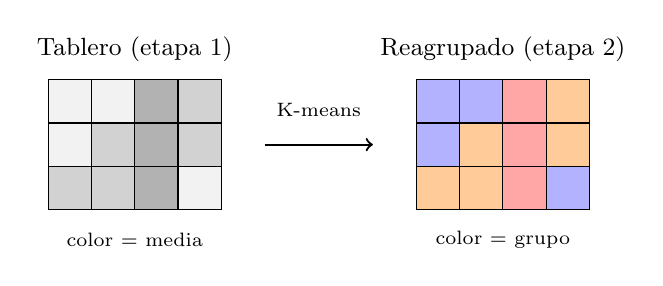
\begin{tikzpicture}[x=0.55cm,y=0.55cm]
    % tablero con la media de cada bloque (niveles de gris)
    \foreach \r/\c/\v in {0/0/10,0/1/10,0/2/60,0/3/35,
                          1/0/10,1/1/35,1/2/60,1/3/35,
                          2/0/35,2/1/35,2/2/60,2/3/10}
      \draw[fill=gray!\v] (\c,-\r) rectangle (\c+1,-\r-1);
    \node at (2,0.7) {\small Tablero (etapa 1)};
    \node at (2,-3.7) {\scriptsize color $=$ media};
    \draw[->, thick] (5,-1.5) -- (7.5,-1.5);
    \node[align=center] at (6.25,-0.7) {\scriptsize K-means};
    % mismos bloques coloreados por grupo de K-means
    \foreach \r/\c/\g in {0/0/blue!30,0/1/blue!30,0/2/red!35,0/3/orange!40,
                          1/0/blue!30,1/1/orange!40,1/2/red!35,1/3/orange!40,
                          2/0/orange!40,2/1/orange!40,2/2/red!35,2/3/blue!30}
      \draw[fill=\g] (\c+8.5,-\r) rectangle (\c+9.5,-\r-1);
    \node at (10.5,0.7) {\small Reagrupado (etapa 2)};
    \node at (10.5,-3.7) {\scriptsize color $=$ grupo};
  \end{tikzpicture}
  \caption{Las dos etapas de ST-CC. A la izquierda, el tablero con el nivel medio de
  cada bloque; a la derecha, los mismos bloques agrupados por K-means. Un grupo
  reúne bloques de distintas filas y columnas, por lo que el resultado ya no es
  una rejilla regular.}
  \label{fig:stcc-etapas}
\end{figure}

\subsection{Lectura de los resultados}

Sobre la partición reagrupada se leen dos tipos de patrón. Un patrón
espacial es la distribución de niveles de actividad sobre todas las regiones
dentro de un grupo de intervalos; como hay cuatro grupos de intervalos, se
obtienen a lo sumo cuatro patrones espaciales por periodo, cuya sucesión a lo
largo del día describe su dinámica temporal. Un patrón temporal es la
secuencia de niveles de actividad que sigue un conjunto de regiones a lo largo
del día; los autores identifican seis patrones temporales en días laborables y
cinco en feriados \cite[Sec.~IV.D]{Liu2021}. Entre los hallazgos, destacan que la
movilidad en días laborables es más dinámica y rítmica, y en feriados más
estática y aleatoria, y que la zona de Penn Station alcanza el nivel de actividad
alto solo en feriados.

\subsection{Limitaciones}\label{sec:stcc-limitaciones}

Tres aspectos del marco motivan directamente esta tesis. Primero, el
reagrupamiento con K-means fusiona bloques del tablero que tienen
media y desviación estándar parecidas, pero no divide ninguno, de modo que la
heterogeneidad que quede dentro de un bloque no se recupera. Segundo, tanto el
número de grupos del tablero como el de K-means se eligen con criterios
heurísticos (la forma de la curva de la función objetivo, el coeficiente de
silueta y el método del codo), sin una interpretación estadística. Tercero, los
propios autores advierten que comparar bloques mediante su media y su desviación
estándar supone que sus distribuciones son semejantes, y que esa condición
debería verificarse antes de aplicar el método \cite[Sec.~IV.E]{Liu2021}. Cada
limitación se corresponde con un elemento de la propuesta del
Capítulo~\ref{chap:propuesta}, de modo que la imposibilidad de dividir bloques se
atiende con el refinamiento jerárquico, los criterios heurísticos con las pruebas
de hipótesis, y el supuesto de distribuciones semejantes con el modelo nulo local
de cada bloque.

\subsection{Base de co-agrupamiento en ST-CC y en esta tesis}\label{sec:stcc-base}

\cite{Liu2021} denominan a su algoritmo \emph{Bregman Block Average
Co-clustering} con I-divergencia, nombre que en \cite[Sec.~3]{Banerjee2007}
corresponde a la base C2. Sin embargo, la función objetivo que declaran es la
pérdida de información mutua $I(R;T) - I(\hat{R};\hat{T})$\footnote{\cite{Liu2021}
escriben $I(R;T) \le I(\hat{R};\hat{T})$. La desigualdad correcta es la inversa,
$I(\hat{R};\hat{T}) \le I(R;T)$, por la desigualdad de procesamiento de datos
\cite{Cover2006}, pues agrupar filas o columnas no puede aumentar la información
mutua.}, que por~\eqref{eq:perdida-im} corresponde a la base C5. La literatura de
la que parte ST-CC describe BBAC\_I como un método que forma co-agrupamientos de
valores similares \cite{Wu2022}, es decir, de bloques constantes, lo que sugiere
que la implementación de \cite{Liu2021} corresponde a C2 aunque la función
objetivo declarada sea la de C5. La implementación pública de BBAC\_I con la que
esta tesis reproduce ST-CC, el paquete \texttt{clustering-geodata-cubes},
corresponde en efecto a C2, ya que aproxima cada bloque por su media y la
divergencia que reporta coincide con la de esa base.

Las dos bases producen un tablero de $K_R \times K_T$ bloques, pero no son
equivalentes. Para una misma partición, la Proposición~\ref{prop:descomposicion} muestra que C5 descuenta
el término (i) y C2 no. Por eso, al optimizar la partición, C2 tiende a agrupar
regiones e intervalos por su volumen, mientras que C5 tiende a agruparlos por la
forma de su perfil.
% DECISIÓN PENDIENTE: confirmar con el asesor la base adoptada. El texto
% siguiente asume C5.
A partir de aquí la subsección deja de describir el trabajo de \cite{Liu2021} y
recoge una decisión de esta tesis, que se retoma en el
Capítulo~\ref{chap:propuesta}. En esta tesis se adopta la base C5. La razón de fondo es que el término (i)
refleja diferencias de volumen entre regiones e intervalos, que no constituyen
interacción espacio-temporal, y C5 lo excluye de la función objetivo; además, es
la función objetivo que \cite{Liu2021} declaran de forma explícita. La base C2,
que probablemente corresponde a su implementación, se reporta como variante en los
experimentos. En ambos casos, el término (iii) de la Proposición~\ref{prop:descomposicion}, sobre el que
actúa el refinamiento, se define igual para una partición dada.

